\documentclass[10pt]{article}
\usepackage[utf8]{inputenc} % utf8 support

% === Document Layout ===
\usepackage[hmargin=1in,vmargin=1in]{geometry}
\usepackage{indentfirst}
\usepackage{lipsum}
\usepackage{url}
\usepackage[colorlinks,linkcolor=red!50!black,citecolor=blue!50!black,urlcolor=blue!50!black]{hyperref}
\usepackage{amsmath}
\usepackage{pdfpages}
\usepackage{physics}
\usepackage{xcolor}
\usepackage{graphicx}
\usepackage{mathtools} % for the coloneq command
\usepackage{xparse}
\usepackage{ifthen} % For checking optional parameters
\usepackage{enumerate}
\usepackage{mathrsfs} % For \mathscr font
\usepackage{amsthm} % The AMS theorems package
\usepackage{amsthm}
\usepackage{tabularx}
\usepackage{authblk} % For affiliations

% amsthm
\newtheorem{theorem}{Theorem}[section]
\newtheorem{corollary}{Corollary}[theorem]
\newtheorem{lemma}[theorem]{Lemma}
\theoremstyle{definition}
\newtheorem{definition}{Definition}[section]
\theoremstyle{remark}
\newtheorem*{remark}{Remark}

\usepackage{amsfonts}
\usepackage{indentfirst}
\usepackage{pgfplots}
\usepackage{tikz}
\usetikzlibrary{
    calc,
    arrows,
    shapes.geometric,
    intersections,
    pgfplots.fillbetween,
    decorations.pathreplacing,
    decorations.markings,
    patterns,
    cd % For commutative diagrams
}
\tikzset{every picture/.style={baseline={([yshift=-0.3em]current bounding box.center)}}}
\tikzset{
    % style to apply some styles to each segment of a path
    on each segment/.style={
        decorate,
        decoration={
            show path construction,
            moveto code={},
            lineto code={
                \path [#1]
                (\tikzinputsegmentfirst) -- (\tikzinputsegmentlast);
            },
            curveto code={
                \path [#1] (\tikzinputsegmentfirst)
                .. controls
                (\tikzinputsegmentsupporta) and (\tikzinputsegmentsupportb)
                ..
                (\tikzinputsegmentlast);
            },
            closepath code={
                \path [#1]
                (\tikzinputsegmentfirst) -- (\tikzinputsegmentlast);
            },
        },
    },
    % style to add short perpendicular bar midway along a path
    bar/.style={
        postaction={
            decorate,
            decoration={
                markings,
                mark=at position .5 with {\arrow{|}}
            }
        }
    }
}

\DeclareMathOperator{\id}{id}
\newcommand{\opcat}{\mathrm{op}}
\DeclareMathOperator{\Hom}{Hom}
\DeclareMathOperator{\cod}{cod}
\DeclareMathOperator{\dom}{dom}

\newcommand{\catA}{\mathcal{A}}
\newcommand{\catB}{\mathcal{B}}
\newcommand{\catC}{\mathcal{C}}
\newcommand{\catD}{\mathcal{D}}
\newcommand{\catE}{\mathcal{E}}

\newcommand{\Pf}{P}

% === Bibliography ===
\usepackage[
    backend=biber,
    style=alphabetic,
]{biblatex}
\addbibresource{references.bib}

\author[1,2]{Thomas C. Fraser}
\author[1]{Tobias Fritz}
\affil[1]{Perimeter Institute for Theoretical Physics, Waterloo, Ontario, Canada, N2L 2Y5}
\affil[2]{Dept. of Physics and Astronomy, University of Waterloo, Waterloo, Ontario, Canada, N2L 3G1}
\date{\today}
\title{On The Bifibrations Underlying Optimization and Elimination}
\begin{document}

\maketitle

\section{Examples}
A prototypical example wherein an adjoint triple 
\[ f_{!}, \exists_{f} \dashv f^{\ast}, f^{-1} \dashv f^{!}, \forall_{f} \]
arises is that of functions $f : X \to Y$ between sets $X$ and $Y$. The inverse image functor $f^{\ast} : \mathscr{P}Y \to \mathscr{P}X$ is defined on a subset $T \subseteq Y$
\[ f^{\ast} ( T ) = \{ x \in X : f(x) \in T \}, \]
and is functorial in the sense that if $T \subseteq T' \subseteq Y$ then $f^{\ast}(T) \subseteq f^{\ast}(T') \subseteq f^{\ast}(T)$. The adjoint functors $\exists_{f}, \forall_{f} : \mathscr{P}X \to \mathscr{P}Y$ are defined on $S \subseteq X$ as
\begin{align*}
    \exists_{f} (S) &= \{ y \in Y : \exists x \in f^{\ast}(y) : x \in S \} \\
    \forall_{f} (S) &= \{ y \in Y : \forall x \in f^{\ast}(y) : x \in S \}
\end{align*}
form an adjoint triple in the sense that $\exists_{f} \dashv f^{\ast} \dashv \forall_{f}$:
\begin{align*}
    \exists_{f} \dashv f^{\ast} : \quad \exists_{f} (S) \subseteq T &\iff S \subseteq f^{\ast}(T) \\
    f^{\ast} \dashv \forall_{f} : \quad f^{\ast}(T) \subseteq R &\iff T \subseteq \forall_{f}(R)
\end{align*}

\begin{center}
    \begin{table}
        \begin{tabular}{|c|c|c|c|c|c|c|}
            \hline
            Context & Fibration & Total $\catE$ & Base $\catE$ & Fibers & Covariant Functor & Contravariant Functor \\
            \hline
            \hline
            Subset Projection & & & & & & \\
            \hline
            Linear Quantifier Elimination & & & & & & \\
            \hline
            Non-linear Quantifier Elimination & & & & & & \\
            \hline
            Real-valued Optimization & & & & & & \\
            \hline
            General Lattice Optimization & & & & & & \\
            \hline
            Convex Projection & & & & & & \\
            \hline
            Convex Optimization & & & & & & \\
            \hline
            Resolution & & & & & & \\
            \hline
            $\ldots$ and more & & & & & & \\
            \hline
        \end{tabular}
    \end{table}
\end{center}

\subsection{Subset Projection}

\begin{center}
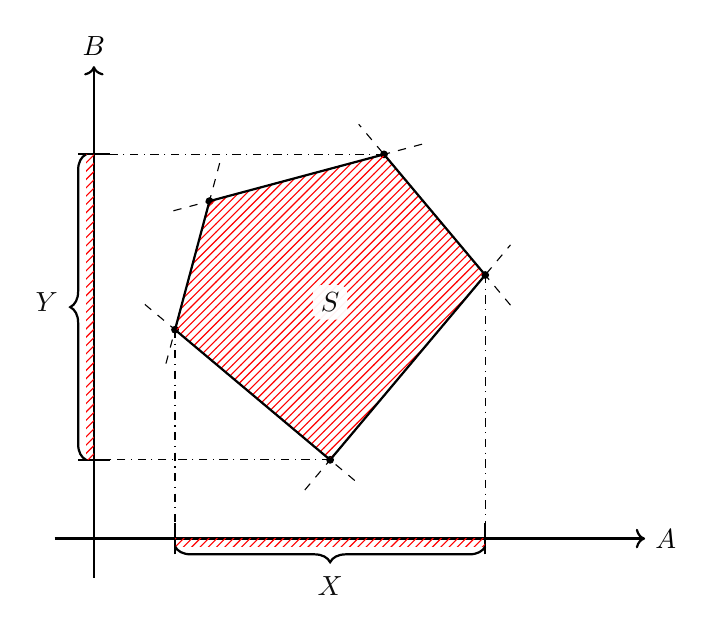
\begin{tikzpicture}[
        extend line/.style={dashed, shorten >= -0.5cm,shorten <= -0.5cm},
        set region/.style={pattern=north east lines, pattern color=red},
        set label/.style={rounded corners=1mm, inner sep=1mm, fill=white, fill opacity=0.95}
    ]
    \coordinate (ori) at (-3,-3);
    \coordinate (A) at ($(ori)+(+7,0)$);
    \coordinate (B) at ($(ori)+(0,+6)$);
    \draw[thick, ->, shorten <= -0.5cm] (ori) -- (A) node[right]{$A$};
    \draw[thick, ->, shorten <= -0.5cm] (ori) -- (B) node[above]{$B$};

    \coordinate (x1) at ( -90:2);
    \coordinate (x2) at ( +10:2);
    \coordinate (x3) at ( +70:2);
    \coordinate (x4) at (+140:2);
    \coordinate (x5) at (+190:2);
    \foreach \p in {x1,x2,x3,x4,x5} {
        \node at (\p)[circle,fill,inner sep=1pt]{}; 
        \coordinate (\p A) at ($(ori)!(\p)!(A)$);
        \coordinate (\p B) at ($(ori)!(\p)!(B)$);
    }
    \draw [thick, set region] (x1) -- (x2) -- (x3) -- (x4) -- (x5) -- cycle;
    \foreach \p/\q in {x1/x2,x2/x3,x3/x4,x4/x5,x5/x1} {
        \draw [extend line] (\p) -- (\q);
    }
    
    \foreach \p in {x2,x5} {
        \draw [dash dot] (\p) -- (\p A);
        \draw [thick] ([yshift=-2mm]\p A) -- ([yshift=+2mm]\p A);
    }
    \path[set region] (x5A) rectangle ([yshift=-1mm]x2A);

    \foreach \p in {x1,x3} {
        \draw [dash dot] (\p) -- (\p B);
        \draw [thick] ([xshift=-2mm]\p B) -- ([xshift=+2mm]\p B);
    }
    \path[set region] (x3B) rectangle ([xshift=-1mm]x1B);
    \node[set label] at (0,0) {$S$};
    \node[set label] at ([yshift=-6mm]$(ori)!(0,0)!(A)$) {$X$};
    \node[set label] at ([xshift=-6mm]$(ori)!(0,0)!(B)$) {$Y$};

    \draw[thick,decorate,decoration={brace,amplitude=2mm}] ([yshift=-1mm]x2A) -- ([yshift=-1mm]x5A);
    \draw[thick,decorate,decoration={brace,amplitude=2mm}] ([xshift=-1mm]x1B) -- ([xshift=-1mm]x3B);
\end{tikzpicture}
\end{center}

\begin{center}
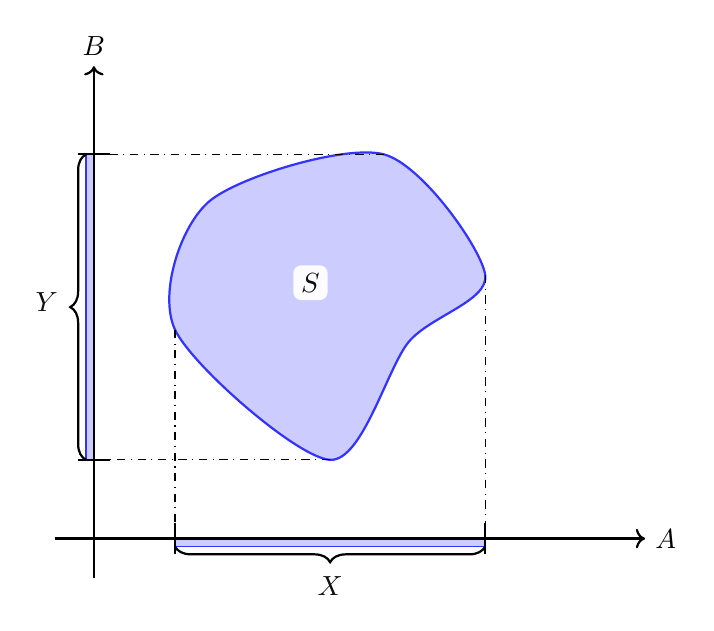
\begin{tikzpicture}[
        set region/.style={draw=blue!80, fill=blue!20},
        set label/.style={rounded corners=1mm, inner sep=1mm, fill=white, fill opacity=0.95}
    ]
    \coordinate (ori) at (-3,-3);
    \coordinate (A) at ($(ori)+(+7,0)$);
    \coordinate (B) at ($(ori)+(0,+6)$);

    \coordinate (x1) at ( -90:2);
    \coordinate (x2) at ( +10:2);
    \coordinate (x3) at ( +70:2);
    \coordinate (x4) at (+140:2);
    \coordinate (x5) at (+190:2);
    \foreach \p in {x1,x2,x3,x4,x5} {
        \coordinate (\p A) at ($(ori)!(\p)!(A)$);
        \coordinate (\p B) at ($(ori)!(\p)!(B)$);
    }
    \draw [thick, set region] plot [smooth cycle] coordinates {(x1) (+1,-0.5) (x2) (x3) (x4) (x5)};
    
    \path[set region] (x5A) rectangle ([yshift=-1mm]x2A);
    \path[set region] (x3B) rectangle ([xshift=-1mm]x1B);

    \foreach \p in {x2,x5} {
        \draw [dash dot] (\p) -- (\p A);
        \draw [thick] ([yshift=-2mm]\p A) -- ([yshift=+2mm]\p A);
    }

    \foreach \p in {x1,x3} {
        \draw [dash dot] (\p) -- (\p B);
        \draw [thick] ([xshift=-2mm]\p B) -- ([xshift=+2mm]\p B);
    }
    \node[set label] at (-0.25,+0.25) {$S$};

    \node[set label] at ([yshift=-6mm]$(ori)!(0,0)!(A)$) {$X$};
    \node[set label] at ([xshift=-6mm]$(ori)!(0,0)!(B)$) {$Y$};

    \draw[thick,decorate,decoration={brace,amplitude=2mm}] ([yshift=-1mm]x2A) -- ([yshift=-1mm]x5A);
    \draw[thick,decorate,decoration={brace,amplitude=2mm}] ([xshift=-1mm]x1B) -- ([xshift=-1mm]x3B);

    \draw[thick, ->, shorten <= -0.5cm] (ori) -- (A) node[right]{$A$};
    \draw[thick, ->, shorten <= -0.5cm] (ori) -- (B) node[above]{$B$};
\end{tikzpicture}
\end{center}

Consider a pair of sets $A$ and $B$ and a subset $S \subseteq A \times B$ of their cartesian product.  The projection morphisms associated with $A \times B$ are $p : A\times B \to A$ and $q : A \times B \to B$. The projection of the subset $S$ onto $A$ is then the subset $X \subseteq A$ defined by:
\[ X = \{ a \in A \mid \exists s \in S, p (s) = a \} \]

\begin{equation}
    S \subseteq p^{\ast} ( X ) \Longleftrightarrow \exists_p ( S ) \subseteq X
\end{equation}

\begin{center}
    \includegraphics[]{figures/min_max_multivariate_function/figure.pdf}
\end{center}

\clearpage
\section{Categorical Notions}

The following unordered list of categorical concepts are anticipated to be utilized:
\begin{itemize}
    \item adjunctions
    \item fibered categories
    \item cleavages
    \item puesdo functors (and if cleavages are splitting, functors)
    \item Beck-Chevalley condition
    \item Frobenius reciprocity (and functors of monoidal categories)
\end{itemize}

\begin{definition}
    Let $P : \catE \to \catB$ be a functor between categories $\catE$ and $\catB$. An arrow $\phi : \alpha \to \beta$ of $\catE$ is \textit{cartesian} with respect to $P$ if for every arrow $\psi : \gamma \to \beta$ sharing a codomain with $\phi$, and for every arrow $g : P(\gamma) \to P(\alpha)$ in $\catB$ satisfying $g \circ P(\phi) = P(\psi)$, there exists a unique arrow $\theta : \gamma \to \alpha$ in $\catE$ satisfying $\phi \circ \theta = \psi$ and $P(\theta) = g$.
    \begin{equation}
        \begin{tikzcd}[row sep=small]
            \gamma \arrow[rd, dashed, "\exists!\theta"'] \arrow[rrd, bend left, "\forall\psi"] \arrow[dd, mapsto] & & \\
            & \alpha \arrow[r, "\phi"'] & \beta \arrow[dd, mapsto] \\
            P(\gamma) \arrow[rd, "\forall g"'] \arrow[rrd, bend left, "P(\psi)"' near start] & & \\
            & P(\alpha) \arrow[r, "P(\phi)"'] \arrow[from=uu, mapsto, crossing over] & P(\beta)
        \end{tikzcd}
    \end{equation}
\end{definition}

\begin{corollary}
    A cartesian morphism $\phi : \alpha \to \beta$ in $\catE$ with respect to a functor $P : \catE \to \catB$ establishes an isomorphism of categories \cite[Section~2.4.1]{lurie2009higher}\footnote{This formulation is also discussed here: \url{https://ncatlab.org/nlab/show/Cartesian+morphism\#CartInOrdCatReformulation}.}
    \begin{equation}
        \catE / \phi \cong \catE / \beta \times_{\catB / P(\beta)} \catB / P(\phi)
    \end{equation}
    where $\catE / \beta \times_{\catB / P(\beta)} \catB / P(\phi)$ is the pullback of functors.
    \begin{equation}
        \begin{tikzcd}
            \catE / \phi \ar[drr, bend left=20, "P/\phi"] \ar[ddr, bend right=40, "\mathrm{cod}"] \ar[dr, dashed, "\cong", leftrightarrow] & & \\ 
            & \catE / \beta \times_{\catB / P(\beta)} \catB / P(\phi) \ar[r] \ar[d] \ar[dr, phantom, "\ulcorner", very near start, xshift=-2em] & \catB / P(\phi) \ar[d, "\mathrm{cod}"] \\ 
            & \catE / \beta \ar[r, "P/\beta"] & \catB / P(\beta) \\ 
        \end{tikzcd}
    \end{equation}
\end{corollary} 
The pullback category $\catE / \beta \times_{\catB / P(\beta)} \catB / P(\phi)$ has morphisms associated with diagrams of $\catB$ with the following format:
\begin{equation}
    \begin{tikzcd}[row sep=large, column sep=small]
        & P(\gamma) \arrow[d, "P(\chi)"] \arrow[ddl, bend right, "f"'] \arrow[ddr, bend left, "P(\omega)"] & \\
        & P(\delta) \arrow[dl, "g"'] \arrow[dr, "P(\psi)"] & \\
        P(\alpha) \arrow[rr, "P(\phi)"] & & P(\beta)
    \end{tikzcd}
    \label{eq:pullback_category_cartesian}
\end{equation}
Evidently, if $\phi : \alpha \to \beta$ is cartesian, then there exists unique morphisms $\zeta : \gamma \to \alpha$ and $\eta : \delta \to \alpha$ such that $P(\zeta) = f$ and $P(\eta) = g$ and the following diagram of $\catE$ commutes:
\begin{equation}
    \begin{tikzcd}[row sep=large]
        & \gamma \arrow[d, "\chi"] \arrow[ddl, bend right, "\zeta"'] \arrow[ddr, bend left, "\omega"] & \\
        & \delta \arrow[dl, "\eta"'] \arrow[dr, "\psi"] & \\
        \alpha \arrow[rr, "\phi"] & & \beta
    \end{tikzcd}
    \label{eq:cartesian_over_category}
\end{equation}
Intuitively, if $\phi$ is cartesian, then in order to determine the category $\catE/\phi$ over $\phi$, it is sufficient to specify $\catE / \beta \times_{\catB / P(\beta)} \catB / P(\phi)$.
\begin{definition}
    A \textit{fibered category over $\catB$} is a category $\catE$ associated to the domain of a functor, referred to as the \textit{fibration}, $P : \catE \to \catB$ with the property that for every morphism $f : a \to b$ of $\catB$ and object $\beta$ such that $P(\beta) = b$, there exists a cartesian arrow $\phi : \alpha \to \beta$ with $P(\phi) = f$.
\end{definition}
\begin{lemma}
    A fibration $P : \catE \to \catB$ is a faithful functor if and only if its fibers are thin.
\end{lemma}
\begin{proof}
    Recall that if $P : \catE \to \catB$ is a faithful functor, then by definition every pair of parallel arrows $\phi, \psi : \alpha \to \beta$ in $\catE$ satisfies 
    \begin{equation}
        \label{eq:faithfulness}
        P(\phi) = P(\psi) : P(\alpha) \to P(\beta) \implies \phi = \psi.
    \end{equation}

    $\implies$ : Assuming $P : \catE \to \catB$ is faithful functor, consider an arbitrary pair of parallel arrows $\phi, \psi : \alpha \to \beta$ in an arbitrary fiber $\catE_{x}$ over $x$; i.e. $P(\phi) = P(\psi) = \id_{x}$. In such cases, faithfulness of $P$ (Eq.~\ref{eq:faithfulness}) guarantees that $\phi = \psi$ and thus $\catE_{x}$ is a thin category.

    $\impliedby$ : If the fiber $\catE_{x}$ for every object $x$ in $\catB$ is a thin category, then clearly $P : \catE \to \catB$ \textit{must} be faithful when restricted to an individual fiber. The non-trivial case is to consider an arbitrary pair of parallel morphisms $\phi, \psi : \alpha \to \beta$ not belonging to any fibers of $\catE$. Denote $a \coloneqq P(\alpha)$ and $b \coloneqq P(\beta)$ and suppose $f \coloneqq P(\phi) = P(\psi) : a \to b$. Then, because $\catE$ is a fibered category, there exists a cartesian arrow $\zeta : \gamma \to \beta$, such that $P(\zeta) = f$ (note that $a = P(\alpha) = P(\gamma)$ but $\gamma$ is not necessarily equal to $\alpha$). Since $\zeta$ is a cartesian arrow, there exists a unique arrows $\mu, \nu: \alpha \to \gamma$ completing the top edges of the following diagram:
    \begin{equation}
        \begin{tikzcd}
            \alpha \ar[dd, mapsto] \ar[rd, "\psi"', bend right] \ar[rr,dashed,"\mu"] & & \gamma \ar[dd, mapsto] \ar[ld, "\zeta"'] & \alpha \ar[dd, mapsto] \ar[lld, "\phi", bend left=20, crossing over, near start] \ar[l, dashed, "\nu"'] \\
            & \beta  & & \\
            a \ar[rr, equals] \ar[rd, "f"', bend right] & & a \ar[r, equals] \ar[ld, "f"] & a \ar[lld,"f", bend left=20] \\
            & b \ar[from=uu, mapsto, crossing over] & & \\
        \end{tikzcd}
        .
    \end{equation}
    However, $P(\nu) = \id_{a} = P(\mu)$ and therefore $\mu$ and $\nu$ are parallel arrows in the fiber $\catE_{a}$ and therefore $\mu = \nu$ because $\catE_{a}$ is assumed thin. Therefore, $\psi = \zeta \circ \mu = \zeta \circ \nu = \phi$ and thus $P$ is a faithful functor.
\end{proof}

\begin{definition}
    A \textit{cleavage} for a fibration $P : \catE \to \catB$ is an assignment to each morphism $f : a \to b$ of $\catB$ and object $\beta$ in $\catE_b$ (i.e. $P(\beta) = b$), a unique cartesian morphism $\phi$ such that $P(\phi) = f$.
\end{definition}

\begin{equation}
    \begin{tikzcd}[column sep=large]
        f^\ast \beta_1 \ar[r, "\kappa(f ; \beta_1)"] & \beta_1 & g^\ast \ar[l, "\kappa(g ; \beta_1)"'] \beta_1 \\
        a \ar[r, "f"] \ar[u, mapsfrom] \ar[d, mapsfrom] & b \ar[u, mapsfrom] \ar[d, mapsfrom] & c \ar[l, "g"'] \ar[u, mapsfrom] \ar[d, mapsfrom] \\
        f^\ast \beta_2 \ar[r, "\kappa(f ; \beta_2)"'] & \beta_2 & g^\ast \beta_2 \ar[l, "\kappa(g ; \beta_2)"]
    \end{tikzcd}
\end{equation}

\section*{Categorical Definitions}

\subsection{Hom-Functors}
For a locally small category $\catC$, the hom-functor of $\catC$ is a functor $\Hom_{\catC} : \catC^{\opcat} \times \catC \to \mathbf{Set}$ constructed in the following manner. Given objects $a,b,c,\ldots \in \catC_0$ of $\catC$, the hom-functor $\Hom_{\catC}$ maps a pair of objects $(a,b) \in (\catC^\opcat \times \catC)_0 = \catC_0 \times \catC_0 = \catC_0^2$ into the set\footnote{The collection of morphisms of type $a \to b$ forms a set because $\catC$ is locally small.} of morphisms $\catC_1$ of $\catC$ with source $a$ and target $b$. Therefore, $\Hom_{\catC}(a,b)$ is the set of morphisms in $\catC$ of type $a \to b$. Given morphisms $g^{\opcat} \in \Hom_{\catC^{\opcat}}(a,c)$ and $h \in \Hom_{\catC}(b,d)$, the hom-functor $\Hom_{\catC}$ constructs a function
\[ \Hom_{\catC}(g^{\opcat}, h) : \Hom_{\catC}(a,b) \to \Hom_{\catC}(c,d) \]
which takes a morphism $f : a \to b \in \Hom_{\catC}(a,b)$ and produces the morphism $h \circ f \circ g : c \to d \in \Hom_{\catC}(c,d)$. Graphically,
\[
    \Hom_{\catC}(g^{\opcat}, h)
    \left(
    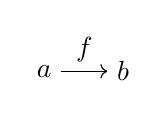
\begin{tikzpicture}
        \draw (0,0) node(a){$a$};
        \draw (1,0) node(b){$b$};
        \draw[->] (a) to node[above, midway]{$f$} (b);
    \end{tikzpicture}
    \right)
    =
    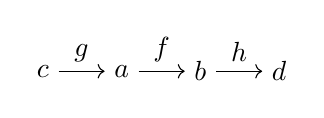
\begin{tikzpicture}
        \draw (0,0) node(c){$c$};
        \draw (1,0) node(a){$a$};
        \draw (2,0) node(b){$b$};
        \draw (3,0) node(d){$d$};
        \draw[->] (c) to node[above, midway]{$g$} (a);
        \draw[->] (a) to node[above, midway]{$f$} (b);
        \draw[->] (b) to node[above, midway]{$h$} (d);
    \end{tikzpicture}
\]

\subsection{Adjoint Functors}
Given two categories $\mathscr{C}$ and $\mathscr{D}$, a pair of functors $L : \mathscr C \to \mathscr D, R : \mathscr D \to \mathscr C$ are called an \textit{adjoint pair}, denoted $L \dashv R$ or
\[
    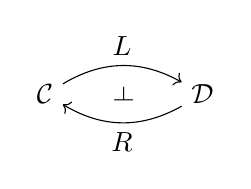
\begin{tikzpicture}
        \draw (0,0) node(c){$\catC$};
        \draw (2,0) node(d){$\catD$};
        \draw[->] (c) to[bend left] node[above, midway]{$L$} (d);
        \draw[->] (d) to[bend left] node[below, midway]{$R$} (c);
        \draw (1,0) node[rotate=-90]{$\dashv$};
    \end{tikzpicture}
\]
if there exists a natural isomorphism $\alpha$ between the following pair of hom-functors of type $\mathscr C^{\opcat} \times \mathscr D \to \mathbf{Set}$:
\[ \Hom_{\mathscr D}(L^{\opcat}(-), -) \stackrel{\alpha}{\simeq} \Hom_{\mathscr C}(-, R(-)) \]
This relationship can be depicted graphically as $2$-cell (and its inverse) in $\mathbf{Cat}$,
\[
    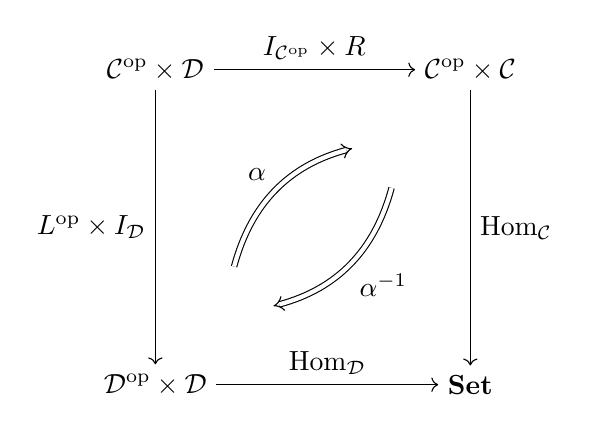
\begin{tikzpicture}
        \draw (0,4) node(tl){$\catC^\opcat \times \catD$};
        \draw (4,4) node(tr){$\catC^\opcat \times \catC$};

        \draw (0,0) node(bl){$\catD^{\opcat} \times \catD$};
        \draw (4,0) node(br){$\mathbf{Set}$};
        \draw[->] (tl) to node[midway, above]{$I_{\catC^{\opcat}} \times R$} (tr);
        \draw[->] (bl) to node[midway, above]{$\Hom_{\catD}$} (br);
        \draw[->] (tl) to node[midway, left]{$L^{\opcat} \times I_{\catD}$} (bl);
        \draw[->] (tr) to node[midway, right]{$\Hom_{\catC}$} (br);

        \draw[double equal sign distance, -implies] (1,1.5) to[bend left] node[above left]{$\alpha$} (2.5,3);
        \draw[double equal sign distance, -implies] (3,2.5) to[bend left] node[below right]{$\alpha^{-1}$} (1.5,1);
    \end{tikzpicture}
\]
Concretely, the naturality of $\alpha$ means that for every morphism $(f^{\opcat} : b \to a, g : c \to d) \in (\catC^{\opcat} \times \catD)_1$ the components $\alpha_{(b,c)}$ and $\alpha_{(a,d)}$ of $\alpha$ make the following square commute:
\[
    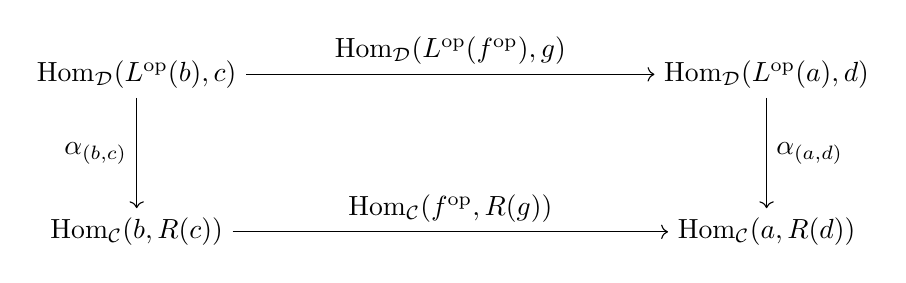
\begin{tikzpicture}
        \draw (0,2) node(tl){$\Hom_{\catD}(L^{\opcat}(b), c)$};
        \draw (8,2) node(tr){$\Hom_{\catD}(L^{\opcat}(a), d)$};
        \draw[->] (tl) to node[midway, above]{$\Hom_{\catD}(L^{\opcat}(f^{\opcat}), g)$} (tr);

        \draw (0,0) node(bl){$\Hom_{\catC}(b, R(c))$};
        \draw (8,0) node(br){$\Hom_{\catC}(a, R(d))$};
        \draw[->] (bl) to node[midway, above]{$\Hom_{\catC}(f^{\opcat}, R(g))$} (br);

        \draw[->] (tl) to node[midway, left]{$\alpha_{(b,c)}$} (bl);
        \draw[->] (tr) to node[midway, right]{$\alpha_{(a,d)}$} (br);
    \end{tikzpicture}
\]

\subsection{Beck-Chevalley Conditions}

The Beck-Chevalley Conditions are conditions that may or may not be satisfied by a quadruplet of functors $F,H,G,K$ which form a natural isomorphism $\alpha : K F \Rightarrow H G$ square:

\[
    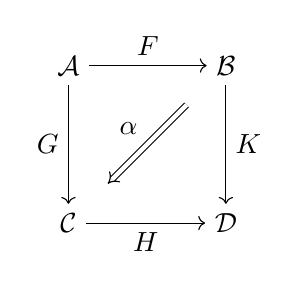
\begin{tikzpicture}
        \draw (-1,+1) node(tl){$\catA$};
        \draw (+1,+1) node(tr){$\catB$};
        \draw (-1,-1) node(bl){$\catC$};
        \draw (+1,-1) node(br){$\catD$};

        \draw[->] (tl) to node[above]{$F$} (tr);
        \draw[->] (tl) to node[left ]{$G$} (bl);
        \draw[->] (bl) to node[below]{$H$} (br);
        \draw[->] (tr) to node[right]{$K$} (br);

        \draw[double equal sign distance, -implies] (+0.5,+0.5) to node[above left]{$\alpha$} (-0.5,-0.5);
    \end{tikzpicture}
\]
To define the \textit{left} Beck-Chevalley condition, one needs functors $F_L : \catB \to \catA$ and $H_L : \catD \to \catA$ which are respectively left adjoint functors to $F$ and $H$, 

\[
    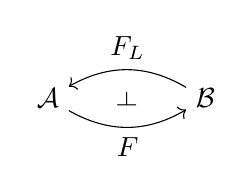
\begin{tikzpicture}
        \draw (-1,+1) node(tl){$\catA$};
        \draw (+1,+1) node(tr){$\catB$};

        \draw[->] (tl) to[bend right] node[below]{$F$} (tr);
        \draw[->] (tr) to[bend right] node[above]{$F_L$} (tl);
        \draw (0,+1) node[rotate=-90]{$\dashv$};
    \end{tikzpicture}
    ,
    \qquad 
    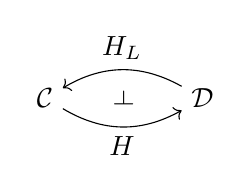
\begin{tikzpicture}
        \draw (-1,-1) node(bl){$\catC$};
        \draw (+1,-1) node(br){$\catD$};

        \draw[->] (bl) to[bend right] node[below]{$H$} (br);
        \draw[->] (br) to[bend right] node[above]{$H_L$} (bl);
        \draw (0,-1) node[rotate=-90]{$\dashv$};
    \end{tikzpicture}
    .
\]
Using these left adjoint functors, it becomes possible to construct a natural transformation $\beta : KH_L \Rightarrow GF_L$ from $\alpha$\footnote{The natural transformations $\alpha$ and $\beta$ are known as \textit{mates} or \textit{conjugates}.}. Graphically, $\beta$ can be identified as the outer cell of the following diagram:
\[
    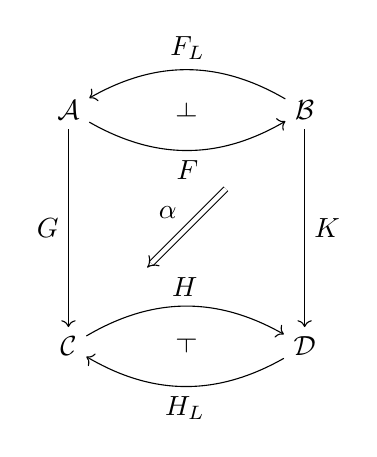
\begin{tikzpicture}
        \draw (-1.5,+1.5) node(tl){$\catA$};
        \draw (+1.5,+1.5) node(tr){$\catB$};
        \draw (-1.5,-1.5) node(bl){$\catC$};
        \draw (+1.5,-1.5) node(br){$\catD$};

        \draw[->] (tl) to[bend right] node[below]{$F$} (tr);
        \draw[->] (tr) to[bend right] node[above]{$F_L$} (tl);
        \draw (0,+1.5) node[rotate=-90]{$\dashv$};
        \draw[->] (tl) to node[left ]{$G$} (bl);
        \draw[->] (bl) to[bend left ] node[above]{$H$} (br);
        \draw[->] (br) to[bend left ] node[below]{$H_L$} (bl);
        \draw (0,-1.5) node[rotate=+90]{$\dashv$};
        \draw[->] (tr) to node[right]{$K$} (br);

        \draw[double equal sign distance, -implies] (+0.5,+0.5) to node[above left]{$\alpha$} (-0.5,-0.5);
    \end{tikzpicture},
    \qquad
    \text{i.e.}
    \qquad
    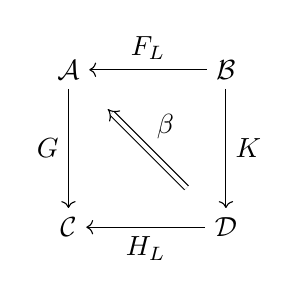
\begin{tikzpicture}
        \draw (-1,+1) node(tl){$\catA$};
        \draw (+1,+1) node(tr){$\catB$};
        \draw (-1,-1) node(bl){$\catC$};
        \draw (+1,-1) node(br){$\catD$};

        \draw[->] (tr) to node[above]{$F_L$} (tl);
        \draw[->] (tl) to node[left ]{$G$} (bl);
        \draw[->] (br) to node[below]{$H_L$} (bl);
        \draw[->] (tr) to node[right]{$K$} (br);

        \draw[double equal sign distance, -implies] (+0.5,-0.5) to node[above right]{$\beta$} (-0.5,+0.5);
    \end{tikzpicture}.
\]
Although the natural transformation $\alpha$ is assumed to be a natural isomorphism, the natural transformation $\beta$ need not be; if $\beta$ happens to be a natural isomorphism, then we say that the original square satisfies the \textit{left} Beck-Chevalley condition\footnote{Are the left adjoints $F_L, H_L$ unique? If not, it might be better to say the original square satifies the left Beck-Chevalley condition with respect to $F_L, H_L$.}. The \textit{right} Beck-Chevalley condition is defined analogously with functors $F_R, H_R$ which are respectively right adjoints $F \dashv F_R$ and $H \dashv H_R$.

\subsection{The Equivalence of Puesdofunctors and Fibrations}

Given a functor $P : \catE \to \catB$ which is also a Grothendieck fibration equipped with a cleavage (i.e. a choice of cartesian morphism $\phi \in \Hom_{\catE}(e', e)$ for each $f \in \Hom_{\catB}(a,P(e))$ such that $P(\phi) = f$), it is possible to construct a pseudofunctor (read weak $2$-functor between weak $2$-categories) $\pi : \catB^{\opcat} \to \mathbf{Cat}$. In particular, each object $b \in \catB_0$ is mapped to the \textit{sub-category} $\pi(b) = \catE_b$ of $\catE$ whose objects are those which map to $b$ under $P$ and whose morphism are those which map to $\id_{b}$ under $P$; $\catE_b$ is the fibre category over $b$ with respect to $P$. For each morphism $f \in \Hom_{\catB}(a,b)$ in $\catB$, the pseudofunctor $\pi$ maps $f^{\opcat} : b \to a$ onto a functor $\pi(f^{\opcat}) = f^{\ast} : \catE_{b} \to \catE_{a}$ which is defined accordingly:
\[
    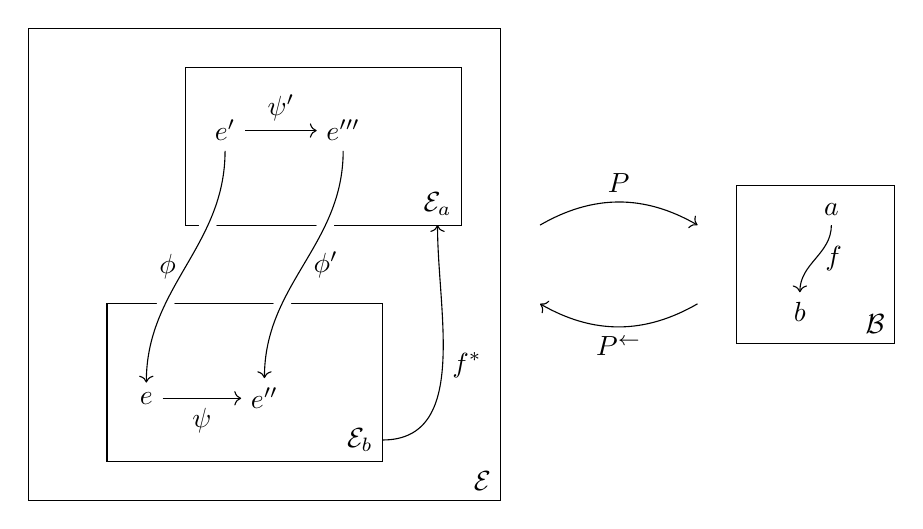
\begin{tikzpicture}
        \begin{scope}[shift={(-4.5,0)}]
            \draw (-3,+3) rectangle (+3,-3) node[above left]{$\catE$};
            \begin{scope}[shift={(-1,+2.5)}]
                \draw (0,0) rectangle (+3.5,-2) node[above left](catEa){$\catE_a$};
                \draw (+0.5, -0.8) node(e2){$e'$};
                \draw (+2, -0.8) node(e4){$e'''$};
                \draw[->] (e2) to node[above]{$\psi'$} (e4);
            \end{scope}
            \begin{scope}[shift={(-2,-0.5)}]
                \draw (0,0) rectangle (+3.5,-2) node[above left](catEb){$\catE_b$};
                \draw (+0.5, -1.2) node(e1){$e$};
                \draw (+2, -1.2) node(e3){$e''$};
                \draw[->] (e1) to node[below]{$\psi$} (e3);
            \end{scope}
            \draw[white, line width=2mm] (e2) to[out=-90,in=+90] (e1);
            \draw[white, line width=2mm] (e4) to[out=-90,in=+90] (e3);
            \draw[->] (e2) to[out=-90,in=+90] node[left ]{$\phi$} (e1);
            \draw[->] (e4) to[out=-90,in=+90] node[right]{$\phi'$} (e3);
            \draw[->] (catEb) to[out=0,in=-90] node[right]{$f^{\ast}$} (catEa);
        \end{scope}
        \begin{scope}[shift={(+1.5,+1)}]
            \draw (0,0) rectangle (+2,-2) node[above left]{$\catB$};
            \draw (+1.2, -0.3) node(a){$a$};
            \draw (+0.8,-1.6) node(b){$b$};
            \draw[->] (a) to[out=-90,in=+90] node[right]{$f$} (b);
        \end{scope}
        \draw[->] (-1,+0.5) to[bend left ] node[above]{$P$} (+1, 0.5);
        \draw[<-] (-1,-0.5) to[bend right] node[below]{$P^{\leftarrow}$} (+1, -0.5);
    \end{tikzpicture}
\]
Given an object $e \in (\catE_b)_0$, the functor $f^{\ast}$ finds the unique cartesian morphism $\phi \in \Hom_{\catE}(e',e)$ as specified by the cleavage and assigns $f^{\ast}(e) = e'$. Next, given a morphism $\psi \in \Hom_{\catE_{b}}(e, e'')$, the functor $f^{\ast}$ first finds the unique cartesian morphisms $\phi \in \Hom_{\catE}(e', e)$ and $\phi' \in \Hom_{\catE}(e''', e'')$. Then, because $g = \id_a$ completes the following diagram
\[
    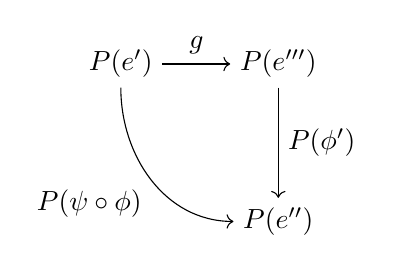
\begin{tikzpicture}
        \draw (-1,+1) node(tl){$P(e')$};
        \draw (+1,+1) node(tr){$P(e''')$};
        \draw (+1,-1) node(br){$P(e'')$};

        \draw[->] (tl) to node[above]{$g$} (tr);
        \draw[->] (tl) to[out=-90, in=180] node[below left]{$P(\psi\circ\phi)$} (br);
        \draw[->] (tr) to node[right]{$P(\phi')$} (br);
    \end{tikzpicture}
    \quad=\quad
    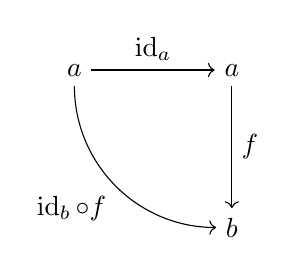
\begin{tikzpicture}
        \draw (-1,+1) node(tl){$a$};
        \draw (+1,+1) node(tr){$a$};
        \draw (+1,-1) node(br){$b$};

        \draw[->] (tl) to node[above]{$\id_{a}$} (tr);
        \draw[->] (tl) to[out=-90, in=180] node[below left]{$\id_{b} \circ f$} (br);
        \draw[->] (tr) to node[right]{$f$} (br);
    \end{tikzpicture},
\]
and because $\phi'$ is cartesian, there must exist a unique $\psi' \in \Hom_{\catE_a}(e', e''')$ such that $\psi \circ \phi = \phi' \circ \psi'$. For each $\psi \in \Hom_{\catE_b}(e, e'')$, the functor $f^{\ast}$ selects this unique morphism $f^{\ast}(\psi) = \psi'$. In summary, the pseudofunctor $\pi : \catB^{\opcat} \to \mathbf{Cat}$ induced by $P : \catE \to \catB$ is defined on objects $b \in \catB_{0}$ as $\pi(b) = \catE_{b}$ and on morphisms $f \in \catB_{1}$ as $\pi(f) = f^{\ast}$ and forms a functor \textcolor{red!50!black}{[TODO: figure out the `pseudo' part of the pseudofunctorality.]}.

\subsection{Slice and Coslice Categories}

Given a category $\catC$ and an object $c \in \catC_0$ of $\catC$, the \textit{slice category} (or \textit{over category}) $\catC/c$ is the ``stuff in $\catC$ that is on top of $c$''. Specifically, the objects of $\catC/c$ are all the morphisms $f \in \catC_1$ from $\catC$ whose codomain is $\cod(f) = c$ (alternatively you could write $(\catC/c)_0 = \Hom_{\catC}(-,c)$). A morphism of $\catC/c$ between objects $f : a \to c, g : b \to c \in (\catC/c)_0$ is a commuting triangle completed by a third morphism $h : a \to b \in \catC_1$:

\[
    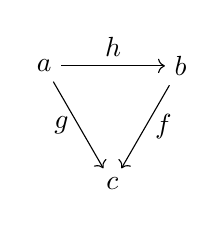
\begin{tikzpicture}
        \draw (150:1) node(tl){$a$};
        \draw ( 30:1) node(tr){$b$};
        \draw (270:1)node(bm){$c$};

        \draw[->] (tl) to node[below,left ]{$g$} (bm);
        \draw[->] (tr) to node[below,right]{$f$} (bm);

        \draw[->] (tl) to node[above]{$h$} (tr);
    \end{tikzpicture}
\]
Composition of morphisms in $\catC/c$ is induced by the composition of morphisms in $\catC$:
\[
    \left(
    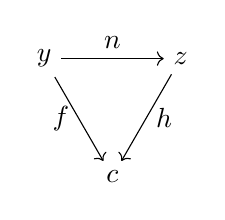
\begin{tikzpicture}
        \draw (150:1) node(tl){$y$};
        \draw ( 30:1) node(tr){$z$};
        \draw (270:1) node(bm){$c$};

        \draw[->] (tl) to node[below,left ]{$f$} (bm);
        \draw[->] (tr) to node[below,right]{$h$} (bm);

        \draw[->] (tl) to node[above]{$n$} (tr);
    \end{tikzpicture}
    \right)
    \circ_{\catC/c}
    \left(
    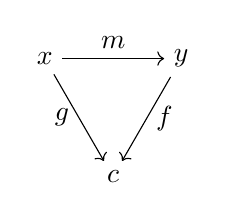
\begin{tikzpicture}
        \draw (150:1) node(tl){$x$};
        \draw ( 30:1) node(tr){$y$};
        \draw (270:1) node(bm){$c$};

        \draw[->] (tl) to node[below,left ]{$g$} (bm);
        \draw[->] (tr) to node[below,right]{$f$} (bm);

        \draw[->] (tl) to node[above]{$m$} (tr);
    \end{tikzpicture}
    \right)
    =
    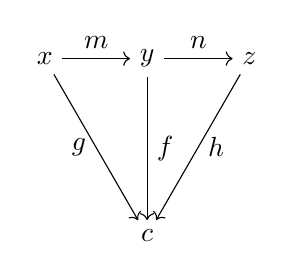
\begin{tikzpicture}
        \draw (150:1.5) node(tl){$x$};
        \draw ( 90:0.75) node(tm){$y$};
        \draw ( 30:1.5) node(tr){$z$};
        \draw (270:1.5) node(bm){$c$};

        \draw[->] (tl) to node[below,left ]{$g$} (bm);
        \draw[->] (tm) to node[right]{$f$} (bm);
        \draw[->] (tr) to node[below,right]{$h$} (bm);

        \draw[->] (tl) to node[above]{$m$} (tm);
        \draw[->] (tm) to node[above]{$n$} (tr);
    \end{tikzpicture}
\]

The assignment of an overcategory $\catC/c$ to each object $c$ can be extended to a \textit{slice functor} $\catC / (-) : \catC \to \mathbf{Cat}$ in the following sense. For objects $c \in \catC_0$, the slice functor takes $c$ to the slice category $\catC/c$; for morphisms $f : a \to b \in \catC_1$, the slice functor takes $f$ to the functor $\catC / f : \catC / a \to \catC / b$ defined graphically; for every morphism of $\catC / a$ (commuting triangle in $\catC$ over $a$), contruct the morphism of $\catC / b$ (commuting triangle in $\catC$ over $b$) as follows:
\[
    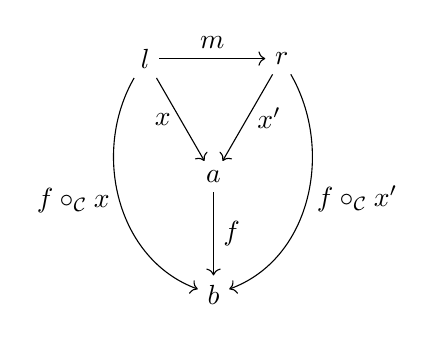
\begin{tikzpicture}
            \draw (150:1) node(tl){$l$};
            \draw ( 30:1) node(tr){$r$};
            \draw (270:1) node(bm){$a$};
            \draw (270:2.5) node(bb){$b$};

            \draw[->] (tl) to node[below,left ]{$x$}  (bm);
            \draw[->] (tr) to node[below,right]{$x'$} (bm);
            \draw[->] (tl) to[out=-120, in=+160] node[below,left ]{$f \circ_{\catC} x$}  (bb);
            \draw[->] (tr) to[out= -60, in= +20] node[below,right]{$f \circ_{\catC} x'$} (bb);
            \draw[->] (tl) to node[above]{$m$} (tr);
            \draw[->] (bm) to node[right]{$f$} (bb);
    \end{tikzpicture}
\]
where the inner triangle is a morphism of $\catC/a$ and the outer triangle is a morphism of $\catC/b$ given by the functor $\catC/f$.

Given a category $\catC$ and an object $c \in \catC_0$ of $\catC$ the \textit{coslice category} (or \textit{under category}) $c/\catC$ is the ``stuff in $\catC$ that is underneath $c$''. Specifically, the objects of $c/\catC$ are all the morphisms $f \in \catC_1$ from $\catC$ whose domain is $\dom(f) = c$ (alternatively you could write $(c/\catC)_0 = \Hom_{\catC}(c,-)$). A morphism of $c/\catC$ between objects $f : c \to a, g : c \to b \in (c/\catC)_0$ is a commuting triangle completed by a third morphism $h : a \to b \in \catC_1$:

\[
    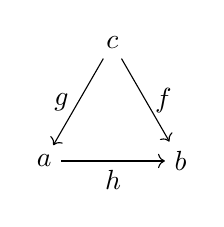
\begin{tikzpicture}
        \draw (210:1) node(tl){$a$};
        \draw (330:1) node(tr){$b$};
        \draw ( 90:1) node(bm){$c$};

        \draw[<-] (tl) to node[below,left ]{$g$} (bm);
        \draw[<-] (tr) to node[below,right]{$f$} (bm);
        \draw[->] (tl) to node[below]{$h$} (tr);
    \end{tikzpicture}
\]
Everything about coslice categories is defined as expected analogously to that of a slice categories.
\textcolor{red!50!black}{[TODO: determine how the details of the Grothendieck construction transform the slice (pseudo-)functor $\catC / (-) : \catC \to \mathbf{Cat}$ into the codomain fibration.]}
\subsection{The Pullback and Pushforward Functors}

Given a category $\catC$ and a morphism $f : a \to b \in \catC_1$, the image of $f$ under the slice functor $\catC / (-)$ produces a functor $\catC / f : \catC / a \to \catC / b$ between slice categories of $\catC$ in the ``same direction'' as $f$ \textcolor{red!50!black}{TODO: confirm that $\catC / f$ is the pushforward functor $f_{!}$ of $f \in \catC_1$.}

If the given category $\catC$ admits pullbacks, in becomes possible to define, for a morphism $f : a \to b$ a pullback functor $f^{*} : \catC / b \to \catC / a$. Given a morphism in $\catC/b$ (commuting triangle in $\catC$ with base at $b$),
\[
    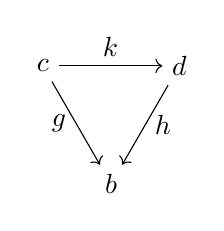
\begin{tikzpicture}
        \begin{scope}[shift={(+3,0)}]
            \draw (150:1) node(ltl){$c$};
            \draw ( 30:1) node(ltr){$d$};
            \draw (270:1) node(lbm){$b$};

            \draw[->] (ltl) to node[below,left ]{$g$}  (lbm);
            \draw[->] (ltr) to node[below,right]{$h$} (lbm);
            \draw[->] (ltl) to node[above]{$k$} (ltr);
        \end{scope}
    \end{tikzpicture}
\]
the pullback functor $f^{\ast} : \catC / b \to \catC / a$ associated with $f$ takes the objects $g : c \to b, h : d \to b$ of $\catC/b$ (morphisms in $\catC$) completes the pullback squares associated with $f$
\[
    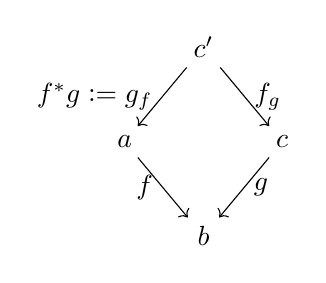
\begin{tikzpicture}
        \begin{scope}[shift={(0,0)}]
            \draw ( 90:1.2) node(t){$c'$};
            \draw (180:1) node(l){$a$};
            \draw (  0:1) node(r){$c$};
            \draw (270:1.2) node(b){$b$};

            \draw[->] (l) to node[below,left ]{$f$} (b);
            \draw[->] (r) to node[below,right]{$g$} (b);
            \draw[->] (t) to node[above,left ]{$f^{\ast}g \vcentcolon= g_{f}$} (l);
            \draw[->] (t) to node[above,right]{$f_{g}$} (r);
        \end{scope}
    \end{tikzpicture}
    \qquad
    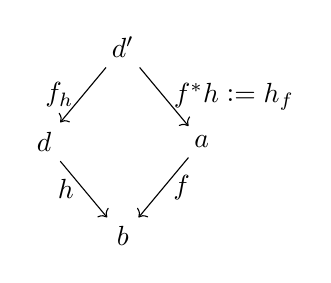
\begin{tikzpicture}
        \begin{scope}[shift={(0,0)}]
            \draw ( 90:1.2) node(t){$d'$};
            \draw (180:1) node(l){$d$};
            \draw (  0:1) node(r){$a$};
            \draw (270:1.2) node(b){$b$};

            \draw[->] (l) to node[below,left ]{$h$} (b);
            \draw[->] (r) to node[below,right]{$f$} (b);
            \draw[->] (t) to node[above,left ]{$f_{h}$} (l);
            \draw[->] (t) to node[above,right]{$f^{\ast}h \vcentcolon= h_{f}$} (r);
        \end{scope}
    \end{tikzpicture}
\]
where a subscript notation $g_{f}$ means ``the pullback of $g$ along $f$''. Defining the action of $f^{\ast} : \catC / b \to \catC / a$ on objects to be $f^{\ast}g = g_{f}$ and $f^{\ast}h = h_{f}$, the action on morphisms in $\catC / b$ is defined by composing the pullback squares with the commuting triangle morphism:
\[
    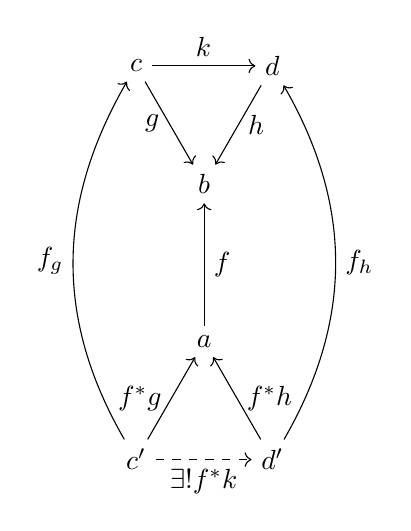
\begin{tikzpicture}
        \begin{scope}[shift={(0,+2)}]
            \draw (150:1) node(t1){$c$};
            \draw ( 30:1) node(t2){$d$};
            \draw (270:1) node(t3){$b$};

            \draw[->] (t1) to node[below,left ]{$g$}  (t3);
            \draw[->] (t2) to node[below,right]{$h$} (t3);
            \draw[->] (t1) to node[above]{$k$} (t2);
        \end{scope}

        \begin{scope}[shift={(0,-2)}]
            \draw (210:1) node(b1){$c'$};
            \draw (330:1) node(b2){$d'$};
            \draw ( 90:1) node(b3){$a$};

            \draw[->] (b1) to node[below,left ]{$f^{\ast}g$} (b3);
            \draw[->] (b2) to node[below,right]{$f^{\ast}h$} (b3);
            \draw[dashed, ->] (b1) to node[below]{$\exists! f^{\ast}k$} (b2);
        \end{scope}
        \draw[->] (b1) to[out=+120, in=-120] node[left ]{$f_{g}$} (t1);
        \draw[->] (b2) to[out=+ 60, in=- 60] node[right]{$f_{h}$} (t2);
        \draw[->] (b3) to node[right]{$f$} (t3);
    \end{tikzpicture}
\]
The commuting triangle in $\catC / a$ appearing at the bottom is completed by a unique morphism \textcolor{red!50!black}{[TODO: why does this morphism need to be unique and exist?]} denoted to be $f^{\ast}k$ ($\neq k_{f}$ obviously). The functoriality of $f^{\ast}$ has a simple proof found here \url{https://proofwiki.org/wiki/Pullback_Functor_is_Functor}.

\subsection{Functors of Monoidal Categories}

\textcolor{red!50!black}{[TODO]}

\subsection{Frobenius Reciprocity}

\textcolor{red!50!black}{[TODO]}

\section*{Comments on selected references}
This section is temporary and reserved for recording comments toward various references.
\begin{itemize}
    \item \citeauthor{vistoli2004notes}~\cite{vistoli2004notes}
    \item \citeauthor{street1974fibrations}~\cite{street1974fibrations}
    \item \citeauthor{koudenburg2018categorical}~\cite{koudenburg2018categorical}
    \item \citeauthor{brown2009algebraic}~\cite{brown2009algebraic}
    \item \citeauthor{lurie2009higher}~\cite{lurie2009higher}
\end{itemize}

\printbibliography
\end{document}
